%% LyX 2.3.4.2 created this file.  For more info, see http://www.lyx.org/.
%% Do not edit unless you really know what you are doing.
\documentclass[english,dvipsnames,aspectratio=169,handout]{beamer}
\usepackage{mathptmx}
\usepackage{eulervm}
\usepackage[T1]{fontenc}
\usepackage[latin9]{inputenc}
\usepackage{babel}
\usepackage{amstext}
\usepackage{amssymb}
\usepackage{graphicx}
\usepackage{ifthen}
\usepackage{xcolor}
\usepackage{xspace}
\usepackage{tikz}
\usetikzlibrary{tikzmark}
\usetikzlibrary{calc}
\usepackage{pgfplots}
%\pgfplotsset{compat=1.17}
\usepackage{booktabs}
\usepackage{bbm}



\ifx\hypersetup\undefined
  \AtBeginDocument{%
    \hypersetup{unicode=true,pdfusetitle,
 bookmarks=true,bookmarksnumbered=false,bookmarksopen=false,
 breaklinks=false,pdfborder={0 0 0},pdfborderstyle={},backref=false,colorlinks=true,
 allcolors=NYUPurple,urlcolor=LightPurple}
  }
\else
  \hypersetup{unicode=true,pdfusetitle,
 bookmarks=true,bookmarksnumbered=false,bookmarksopen=false,
 breaklinks=false,pdfborder={0 0 0},pdfborderstyle={},backref=false,colorlinks=true,
 allcolors=NYUPurple,urlcolor=LightPurple}
\fi

\makeatletter

%%%%%%%%%%%%%%%%%%%%%%%%%%%%%% LyX specific LaTeX commands.
%% Because html converters don't know tabularnewline
\providecommand{\tabularnewline}{\\}

%%%%%%%%%%%%%%%%%%%%%%%%%%%%%% Textclass specific LaTeX commands.
% this default might be overridden by plain title style
\newcommand\makebeamertitle{\frame{\maketitle}}%
% (ERT) argument for the TOC
\AtBeginDocument{%
  \let\origtableofcontents=\tableofcontents
  \def\tableofcontents{\@ifnextchar[{\origtableofcontents}{\gobbletableofcontents}}
  \def\gobbletableofcontents#1{\origtableofcontents}
}

%%%%%%%%%%%%%%%%%%%%%%%%%%%%%% User specified LaTeX commands.
\usetheme{CambridgeUS} 
\beamertemplatenavigationsymbolsempty


% Set Color ==============================
\definecolor{NYUPurple}{RGB}{87,6,140}
\definecolor{LightPurple}{RGB}{165,11,255}


\setbeamercolor{title}{fg=NYUPurple}
\setbeamercolor{frametitle}{fg=NYUPurple}

\setbeamercolor{background canvas}{fg=NYUPurple, bg=white}
\setbeamercolor{background}{fg=black, bg=NYUPurple}

\setbeamercolor{palette primary}{fg=black, bg=gray!30!white}
\setbeamercolor{palette secondary}{fg=black, bg=gray!20!white}
\setbeamercolor{palette tertiary}{fg=gray!20!white, bg=NYUPurple}

\setbeamertemplate{headline}{}
\setbeamerfont{itemize/enumerate body}{}
\setbeamerfont{itemize/enumerate subbody}{size=\normalsize}

\setbeamercolor{parttitle}{fg=NYUPurple}
\setbeamercolor{sectiontitle}{fg=NYUPurple}
\setbeamercolor{sectionname}{fg=NYUPurple}
\setbeamercolor{section page}{fg=NYUPurple}
%\setbeamercolor{description item}{fg=NYUPurple}
%\setbeamercolor{block title}{fg=NYUPurple}

\setbeamertemplate{blocks}[rounded][shadow=false]
\setbeamercolor{block body}{bg=normal text.bg!90!NYUPurple}
\setbeamercolor{block title}{bg=NYUPurple!30, fg=NYUPurple}



\AtBeginSection[]{
  \begin{frame}
  \vfill
  \centering
\setbeamercolor{section title}{fg=NYUPurple}
 \begin{beamercolorbox}[sep=8pt,center,shadow=true,rounded=true]{title}
    \usebeamerfont{title}\usebeamercolor[fg]{title}\insertsectionhead\par%
  \end{beamercolorbox}
  \vfill
  \end{frame}
}

\makeatother

\setlength{\parskip}{\medskipamount} 

\input ../macros

\begin{document}
\input ../rosenberg-macros

\title[CSCI-GA 2565]{Kernels \& Probabilistic Modeling}
\author{Mengye Ren}
\date{October 3, 2023}
\institute{NYU}

\makebeamertitle
\mode<article>{Just in article version}


\begin{frame}{Logistics}
\begin{itemize}
    \item Oct 10 (next week): Legislative Day No Class
    \item Oct 17: Homework 2 Due
    \item Oct 24: Midterm, in class, covers everything up until Oct 17
\end{itemize}
\end{frame}

% \section{Kernelization}

\begin{frame}{Dual Problem: Dependence on $x$ through inner products}
\begin{itemize}
\item SVM Dual Problem:
\begin{eqnarray*}
\sup_{\alpha} &  & \sum_{i=1}^{n}\alpha_{i}-\frac{1}{2}\sum_{i,j=1}^{n}\alpha_{i}\alpha_{j}y_{i}y_{j}x_{j}^{T}x_{i}\\
\mbox{s.t.} &  & \sum_{i=1}^{n}\alpha_{i}y_{i}=0\\
 & \quad & \alpha_{i}\in\left[0,\frac{c}{n}\right]\;i=1,\ldots,n.
\end{eqnarray*}


\item Note that all dependence on inputs $x_{i}$ and $x_{j}$ is through
their inner product: $\left\langle x_{j},x_{i}\right\rangle =x_{j}^{T}x_{i}$.

\item We can replace $x_{j}^{T}x_{i}$ by other products... 

\item This is a ``kernelized'' objective function. 
\end{itemize}
\end{frame}


\section{Feature Maps}

\begin{frame}{The Input Space $\cx$}
\begin{itemize}
\item Our general learning theory setup: no assumptions about $\cx$

\item But $\cx=\reals^{d}$ for the specific methods we've developed: 
\begin{itemize}
\item Ridge regression
\item Lasso regression
\item Support Vector Machines 
\end{itemize}
\item Our hypothesis space for these was all affine functions on $\reals^{d}$:
\[
\cf=\left\{ x\mapsto w^{T}x+b\mid w\in\reals^{d},b\in\reals\right\} .
\]
\item What if we want to do prediction on inputs not natively in $\reals^{d}$?
\end{itemize}
\end{frame}
%

\begin{frame}{The Input Space $\cx$}
\begin{itemize}
\item Often want to use inputs not natively in $\reals^{d}$:
\begin{itemize}
\item Text documents
\item Image files
\item Sound recordings
\item DNA sequences
\end{itemize}
\pause
\item They may be represented in numbers, but... 
\item The $i$th entry of each sequence should have the same ``meaning''
\item All the sequences should have the same length
\end{itemize}
\end{frame}

\begin{frame}{Feature Extraction}
\begin{definition}
Mapping an input from $\cx$ to a vector in $\reals^{d}$ is called
\textbf{feature extraction} or \textbf{featurization}. 
\end{definition}

\begin{center}
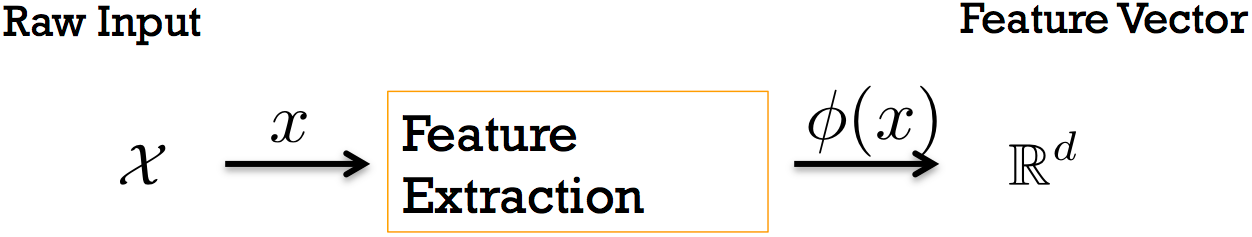
\includegraphics[width=0.9\textwidth]{figures/feature-extraction}
\par\end{center}

\end{frame}

\begin{frame}{Linear Models with Explicit Feature Map}
\begin{itemize}
\item Input space: $\cx$ (no assumptions)
\item Introduce \textbf{feature map} $\phi:\cx\to\reals^{d}$
\item The feature map maps into the \textbf{feature space} $\reals^{d}$.
\pause
\item Hypothesis space of affine functions on feature space:
\[
    \cf=\left\{ x\mapsto w^{T}{\color{blue}\phi(x)}+b\mid w\in\reals^{d},b\in\reals\right\} .
\]
\end{itemize}
\end{frame}
%
\begin{frame}{Geometric Example: Two class problem, nonlinear boundary}
\begin{center}
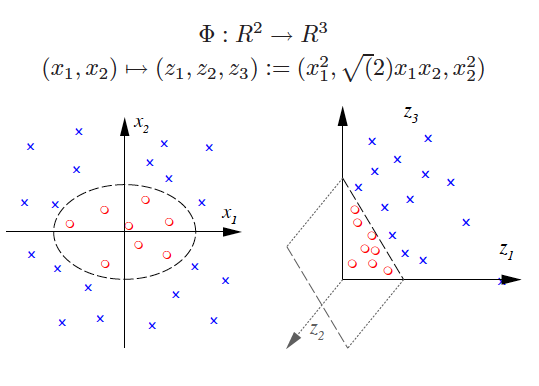
\includegraphics[height=0.6\textheight]{figures/feature-map-3d}
\par\end{center}
    \vspace{-1em}
\begin{itemize}
\item With identity feature map $\phi(x)=\left(x_{1},x_{2}\right)$ and
linear models, can't separate regions

\item With appropriate featurization $\phi(x)=\left(x_{1},x_{2},x_{1}^{2}+x_{2}^{2}\right)$,
becomes linearly separable . 

\item Video: \url{http://youtu.be/3liCbRZPrZA} 
\end{itemize}
    % \let\thefootnote\relax\footnotetext{\tiny{\url{https://math.stackexchange.com/questions/353607/how-do-inner-product-space-determine-half-planes}}}
\end{frame}
%
\begin{frame}{Expressivity of Hypothesis Space}
\begin{itemize}
\item For linear models, to grow the hypothesis spaces, we must add features.

\item Sometimes we say a larger hypothesis is \hl{more expressive}. 
\begin{itemize}
\item (can fit more relationships between input and action)
\end{itemize}

\item Many ways to create new features.
\end{itemize}
\end{frame}
%

\section{Handling Nonlinearity with Linear Methods}
\begin{frame}{Example Task: Predicting Health}
\begin{itemize}
\item General Philosophy: Extract every feature that might be relevant

\item Features for medical diagnosis
\begin{itemize}
\item height
\item weight
\item body temperature
\item blood pressure
\item etc...
\end{itemize}
\end{itemize}
\let\thefootnote\relax\footnotetext{\tiny{From Percy Liang's "Lecture 3" slides from Stanford's CS221, Autumn 2014. }}
\end{frame}

\begin{frame}{Feature Issues for Linear Predictors}
\begin{itemize}
\item For linear predictors, it's important \textbf{how} features are added
    \begin{itemize}
        \item The relation between a feature and the label may not be linear
        \item There may be complex dependence among features
    \end{itemize}

\pause
\item Three types of nonlinearities can cause problems:

\begin{itemize}
\item Non-monotonicity
\item Saturation
\item Interactions between features
\end{itemize}
\end{itemize}
\let\thefootnote\relax\footnotetext{\tiny{From Percy Liang's "Lecture 3" slides from Stanford's CS221, Autumn 2014. }}
\end{frame}

\begin{frame}{Non-monotonicity: The Issue}
\begin{itemize}
\item Feature Map: $\phi(x)=\left[1,\text{temperature}(x)\right]$

\item Action: Predict health score $y\in\reals$ (positive is good)

\item Hypothesis Space $\cf{=}\left\{ \mbox{affine functions of temperature}\right\} $

\pause
\item Issue: 

\begin{itemize}
\item Health is not an affine function of temperature.

\pause
\item Affine function can either say
\begin{itemize}
\item Very high is bad and very low is good, or
\item Very low is bad and very high is good,
\item But here, both extremes are bad.
\end{itemize}
\end{itemize}
\end{itemize}
\let\thefootnote\relax\footnotetext{\tiny{From Percy Liang's "Lecture 3" slides from Stanford's CS221, Autumn 2014. }}
\end{frame}

\begin{frame}{Non-monotonicity: Solution 1}
\begin{itemize}
\item Transform the input:
\[
\phi(x)=\left[1,\left\{ \text{temperature(x)-37}\right\} ^{2}\right],
\]
where $37$ is ``normal'' temperature in Celsius.
\pause

\item Ok, but requires manually-specified domain knowledge
\begin{itemize}
\item Do we really need that?
\item What does $w^T\phi(x)$ look like?
\end{itemize}
\end{itemize}
\let\thefootnote\relax\footnotetext{\tiny{From Percy Liang's "Lecture 3" slides from Stanford's CS221, Autumn 2014. }}
\end{frame}

\begin{frame}{Non-monotonicity: Solution 2}
\begin{itemize}
\item Think less, put in more:
\[
\phi(x)=\left[1,\text{temperature}(x),\left\{ \text{temperature}(x)\right\} ^{2}\right].
\]


\item \hl{More expressive} than Solution 1.

\end{itemize}
\begin{block}{General Rule}

Features should be simple building blocks that can be pieced together.
\end{block}
\let\thefootnote\relax\footnotetext{\tiny{From Percy Liang's "Lecture 3" slides from Stanford's CS221, Autumn 2014. }}
\end{frame}

\begin{frame}{Saturation: The Issue}
\begin{itemize}
\item Setting: Find products relevant to user's query

\pause
\item Input: Product $x$
\item Output: Score the relevance of $x$ to user's query

\pause
\item Feature Map:
\[
\phi(x)=\left[1,N(x)\right],
\]
where $N(x)=\text{number of people who bought }x$.

\pause
\item We expect a monotonic relationship between $N(x)$ and relevance,
    but also expect \hl{diminishing return}.
\end{itemize}
\let\thefootnote\relax\footnotetext{\tiny{From Percy Liang's "Lecture 3" slides from Stanford's CS221, Autumn 2014. }}
\end{frame}

\begin{frame}{Saturation: Solve with nonlinear transform}
\begin{itemize}
\item Smooth nonlinear transformation:
\[
\phi(x)=\left[1,\log\left\{ 1+N(x)\right\} \right]
\]

\begin{itemize}
    \item $\log\left(\cdot\right)$ good for values with large dynamic ranges
\end{itemize}
\pause
\item Discretization (a discontinuous transformation):
\[
\phi(x)=\left(\ind{0\le N(x)<10},\ind{10\le N(x)<100},\ldots\right)
\]

        \begin{itemize}
\item Small buckets allow quite flexible relationship
\end{itemize}

\end{itemize}

\let\thefootnote\relax\footnotetext{\tiny{From Percy Liang's "Lecture 3" slides from Stanford's CS221, Autumn 2014. }}
\end{frame}

\begin{frame}{Interactions: The Issue}
\begin{itemize}
\item Input: Patient information $x$
\item Action: Health score $y\in\reals$ (higher is better)
\item Feature Map
\[
\phi(x)=\left[\mbox{height}(x),\mbox{weight}(x)\right]
\]

\pause
\item Issue: It's the weight \textit{relative} to the height that's important.

\pause
\item Impossible to get with these features and a linear classifier.
\item Need some \textbf{interaction} between height and weight.

\let\thefootnote\relax\footnotetext{\tiny{From Percy Liang's "Lecture 3" slides from Stanford's CS221, Autumn 2014. }}
\end{itemize}
\end{frame}

\begin{frame}{Interactions: Approach 1}
\begin{itemize}
\item Google ``ideal weight from height''

\item J. D. Robinson's ``ideal weight'' formula:
 % (for a male):
\[
\mbox{weight}\mbox{(kg)}=52+1.9\left[\mbox{height(in)}-60\right]
\]

\pause
\item Make score square deviation between height($h$) and ideal weight($w$)
\[
f(x)=\left(52+1.9\left[h(x)-60\right]-w(x)\right)^{2}
\]

\pause
\item WolframAlpha for complicated Mathematics:
\[
f(x)=3.61h(x)^{2}-3.8h(x)w(x)-235.6h(x)+w(x)^{2}+124w(x)+3844
\]
\end{itemize}
\let\thefootnote\relax\footnotetext{\tiny{From Percy Liang's "Lecture 3" slides from Stanford's CS221, Autumn 2014. }}
\end{frame}

\begin{frame}{Interactions: Approach 2}
\begin{itemize}
\item Just include all second order features:
\[
\phi(x)=\left[1,h(x),w(x),h(x)^{2},w(x)^{2},\underbrace{h(x)w(x)}_{\mbox{cross term}}\right]
\]

\item More flexible, no Google, no WolframAlpha.
\end{itemize}
\begin{block}{General Principle}

Simpler building blocks replace a single ``smart'' feature.
\end{block}
\let\thefootnote\relax\footnotetext{\tiny{From Percy Liang's "Lecture 3" slides from Stanford's CS221, Autumn 2014. }}
\end{frame}

%\begin{frame}{Predicate Features and Interaction Terms}
%\begin{definition}
%A \textbf{predicate} on the input space $\cx$ is a function $P:\cx\to\left\{ \mbox{True},\mbox{False}\right\} $.
%
%\pause{}
%\end{definition}
%
%\begin{itemize}
%\item Many features take this form:
%\begin{itemize}
%\item $x\mapsto s(x)=\ind{\mbox{subject is sleeping}}$
%\item $x\mapsto d(x)=\ind{\mbox{subject is driving}}$
%
%\pause{}
%\end{itemize}
%\item For predicates, interaction terms correspond to \textbf{AND} conjunctions:
%\begin{itemize}
%\item $x\mapsto s(x)d(x)=\ind{\mbox{subject is sleeping AND subject is driving}}$
%\end{itemize}
%\end{itemize}
%\let\thefootnote\relax\footnotetext{\tiny{From Percy Liang's "Lecture 3" slides from Stanford's CS221, Autumn 2014. }}
%\end{frame}

\begin{frame}{Monomial Interaction Terms}
    \textbf{Interaction terms} are useful building blocks to model non-linearities in features.
\begin{itemize}
\item Suppose we start with $x=\left(1,x_{1},\ldots,x_{d}\right)\in\reals^{d+1}=\cx$.

\pause
\item Consider adding all \textbf{monomials} of degree $M$: $x_{1}^{p_{1}}\cdots x_{d}^{p_{d}}$,
with $p_{1}+\cdots+p_{d}=M$.

        \begin{itemize}
            \item Monomials with degree 2 in 2D space: $x_1^2$, $x_2^2$, $x_1x_2$
        \end{itemize}

\pause
\item How many features will we end up with? 
\pause
\begin{center}
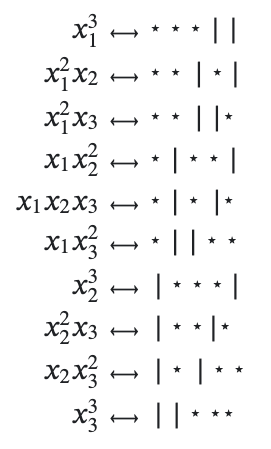
\includegraphics[width=0.2\textwidth]{figures/star-and-bar.png}
\end{center}
\pause
${M+d-1 \choose M}$
% (``stars and bars'')
    % \pdfnote{Distribute M degrees/objects to d boxes. Place (n-1) bars among M indistinguishable objects.}
% \item This leads to extremely \al{large data matrices}
% \begin{itemize}
% \item For $d=40$ and $M=8$, we get $314457495$ features.
% \end{itemize}
\end{itemize}
\end{frame}

\begin{frame}{Big Feature Spaces}
This leads to extremely \al{large data matrices}
\begin{itemize}
\item For $d=40$ and $M=8$, we get $314457495$ features.
\end{itemize}

\pause
Very large feature spaces have two potential issues:\\
\begin{itemize}
\item Overfitting
\item Memory and computational costs 
\end{itemize}

\pause
    Solutions:\\
\begin{itemize}
\item Overfitting we handle with regularization.
\item \textbf{Kernel methods} can help with memory and
    computational costs when we go to high (or infinite) dimensional spaces.
\end{itemize}
\end{frame}

\section{The Kernel Trick}

\begin{frame}{SVM with Explicit Feature Map}
\begin{itemize}
\item Let $\psi:\cx\to\reals^{d}$ be a feature map.

\item The SVM objective (with explicit feature map):
\[
\min_{w\in\reals^{d}}\frac{1}{2}||w||^{2}+\frac{c}{n}\sum_{i=1}^{n}\max\left(0,1-y_{i}w^{T}\psi(x_{i})\right).
\]
\pause
\item Computation is costly if $d$ is large (e.g. with high-degree monomials)
\pause
\item Last time we mentioned an equivalent optimization problem from Lagrangian
duality.
\end{itemize}
\end{frame}
%
\begin{frame}{SVM Dual Problem}
\begin{itemize}
\item By Lagrangian duality, it is equivalent to solve the following dual problem:
\end{itemize}
\begin{eqnarray*}
    \text{maximize} &  & \sum_{i=1}^{n}\alpha_{i}-\frac{1}{2}\sum_{i,j=1}^{n}\alpha_{i}\alpha_{j}y_{i}y_{j}
    {\color{blue}\psi\left(x_{j}\right)^{T}\psi(x_{i})}\\
\mbox{s.t.} &  & \sum_{i=1}^{n}\alpha_{i}y_{i}=0\qquad\text{and}\qquad\alpha_{i}\in\left[0,\frac{c}{n}\right]\quad\forall i.
\end{eqnarray*}

\begin{itemize}
\item If $\alpha^{*}$ is an optimal value, then
\[
w^{*}=\sum_{i=1}^{n}\alpha_{i}^{*}y_{i}\psi(x_{i})\qquad\text{and}\qquad\hat{f}(x)=\sum_{i=1}^{n}\alpha_{i}^{*}y_{i}
        {\color{blue}\psi(x_{i})^{T}\psi(x)}.
\]
\end{itemize}

\pause
\begin{itemize}
    \item \head{Key observation}: $\psi\left(x\right)$ only shows up in \hl{inner products} with
        another $\psi(x')$ \emph{for both training and inference}.
\end{itemize}
\end{frame}
%
\begin{frame}
    {Compute the Inner Products}
    Consider 2D data. Let's introduce \hl{degree-2 monomials} using $\psi:\reals^2\rightarrow\reals^3$.
    $$
    (x_1, x_2) \mapsto (x_1^2, \sqrt{2}x_1x_2, x_2^2) .
    $$
    The inner product is
    \begin{align*}
        \psi(x)^T\psi(x') &= x_{1}^2 {x'_{1}}^2 +
        (\sqrt{2}x_{1}x_{2})(\sqrt{2}x'_{1}x'_{2}) +
        x_{2}^2 {x'_{2}}^2 \\
        &= (x_{1} x'_{1})^2 + 2(x_{1} x'_{1})(x_{2} x'_{2}) + (x_{2} x'_{2})^2 \\
        &= (x_{1}x'_{1} + x_{2}x'_{2})^2 \\
        &= (x^Tx')^2
    \end{align*}
    We can calculate the inner product $\psi(x)^T\psi(x')$ in the original input space without accessing the features $\psi(x)$!
\end{frame}
%
\begin{frame}
    {Compute the Inner Products}
    Now, consider \hl{monomials up to degree-2}:
    $$
    (x_1, x_2) \mapsto (1, \sqrt{2}x_1, \sqrt{2}x_2, x_1^2, \sqrt{2}x_1x_2, x_2^2) .
    $$
    The inner product can be computed by
    $$
    \psi(x)^T\psi(x') = (1 + x^Tx')^2 \quad \text{(check)}.
    $$
    More generally, for features maps producing monomials up to degree-$p$, we have
    $$
    \psi(x)^T\psi(x') = (1 + x^Tx')^p . 
    $$
    (Note that the coefficients of each monomial in $\psi$ may not be 1)

    \textbf{Kernel trick}: we do not need explicit features to calculate inner products.
    \begin{itemize}
        \setlength\itemsep{1ex}
        \item Using explicit features: $O(d^p)$
        \item Using implicit computation: $O(d)$
    \end{itemize}
\end{frame}
%
\section{Kernel Function}
\begin{frame}{The Kernel Function}
\begin{itemize}
    \setlength\itemsep{1ex}
\item \textbf{Input space}: $\cx$

\item \textbf{Feature space}: $\ch$ (a Hilbert space, e.g. $\reals^{d}$)

\item \textbf{Feature map}: $\psi:\cx\to\ch$

\item The \textbf{kernel function} corresponding to $\psi$ is 
\[
k(x,x')=\left\langle \psi(x),\psi(x')\right\rangle ,
\]
where $\left\langle \cdot,\cdot\right\rangle $ is the inner product
associated with $\ch$.
\end{itemize}

\pause
Why introduce this new notation $k(x,x')$?

\pause
\begin{itemize}
    \item We can often evaluate $k(x,x')$ without explicitly computing $\psi(x)$ and $\psi(x')$.
\end{itemize}

\pause
When can we use the kernel trick?
\end{frame}
%
\begin{frame}{Some Methods Can Be ``Kernelized''}
\begin{definition}
A method is \textbf{kernelized }if every feature vector $\psi(x)$
only appears inside an inner product with another feature vector $\psi(x')$.
This applies to both the optimization problem and the prediction function.
\end{definition}
\pause

The SVM Dual is a kernelization of the original SVM formulation. 

Optimization:
    \vspace{-1ex}
\begin{eqnarray*}
    \text{maximize} &  & \sum_{i=1}^{n}\alpha_{i}-\frac{1}{2}\sum_{i,j=1}^{n}\alpha_{i}\alpha_{j}y_{i}y_{j}
    {\color{blue}\psi\left(x_{j}\right)^{T}\psi(x_{i})}\\
\mbox{s.t.} &  & \sum_{i=1}^{n}\alpha_{i}y_{i}=0\qquad\text{and}\qquad\alpha_{i}\in\left[0,\frac{c}{n}\right]\quad\forall i.
\end{eqnarray*}

Prediction:
    \vspace{-1ex}
\[
\hat{f}(x)=\sum_{i=1}^{n}\alpha_{i}^{*}y_{i}
        {\color{blue}\psi(x_{i})^{T}\psi(x)}.
\]

\end{frame}
%
\begin{frame}{The Kernel Matrix}
\begin{definition}
The \textbf{kernel matrix} for a kernel $k$ on $x_{1},\ldots,x_{n}\in\cx$
is
\[
K=\begin{pmatrix}k(x_{i},x_{j})\end{pmatrix}_{i,j}=\begin{pmatrix}k(x_{1},x_{1}) & \cdots & k(x_{1},x_{n})\\
\vdots & \ddots & \cdots\\
k(x_{n},x_{1}) & \cdots & k(x_{n},x_{n})
\end{pmatrix}\in\reals^{n\times n}.
\]
\end{definition}

\begin{itemize}
\item In ML this is also called a \textbf{Gram matrix}, but traditionally
(in linear algebra),
Gram matrices are defined without reference to a kernel or feature
map.
\end{itemize}
\end{frame}
%
\begin{frame}{The Kernel Matrix}
\begin{itemize}
    \item The kernel matrix \hl{summarizes all the information} we need about the
training inputs $x_{1},\ldots,x_{n}$ to solve a kernelized optimization
problem.
\item In the kernelized SVM, we can replace $\psi(x_{i})^{T}\psi(x_{j})$
with $K_{ij}$:
\begin{eqnarray*}
    \text{maximize}_{\alpha} &  & \sum_{i=1}^{n}\alpha_{i}-\frac{1}{2}\sum_{i,j=1}^{n}\alpha_{i}\alpha_{j}y_{i}y_{j}{\color{blue}K_{ij}}\\
\mbox{s.t.} &  & \sum_{i=1}^{n}\alpha_{i}y_{i}=0\qquad\text{and}\qquad\alpha_{i}\in\left[0,\frac{c}{n}\right]\;i=1,\ldots,n.
\end{eqnarray*}
\end{itemize}
\end{frame}
%
\begin{frame}{Kernel Methods}
Given a kernelized ML algorithm (i.e. all $\psi(x)$'s show up as
$\left\langle \psi(x),\psi(x')\right\rangle $),

\begin{itemize}

\item Can swap out the inner product for a new kernel function.

\item New kernel may correspond to a \al{very high-dimensional} feature space.

\pause

\item Once the kernel matrix is computed, the computational cost \hl{depends
    on number of data points} $n$, rather than the dimension of feature space $d$.

\item Useful when $d >> n$.

\pause

\item Computing the kernel matrix may still depend on $d$
    and the essence of the \textbf{trick} is getting around this $O(d)$ dependence.
\end{itemize}
\end{frame}
%
\section{Example Kernels}
\begin{frame}{Kernels as Similarity Scores}
\begin{itemize}
    \item Often useful to think of the $k(x, x')$ as a \textbf{similarity
score} for $x$ and $x'$.
\item We can design similarity functions without thinking about the explicit feature map, e.g. ``string kernels'', ``graph kernels''.
\item How do we know that our kernel functions actually correspond to inner products in
    some feature space?
\end{itemize}
\end{frame}
%
\begin{frame}{How to Get Kernels?}
\begin{itemize}
    \item Explicitly construct $\psi(x):\cx\to\reals^{d}$ (e.g. monomials) and define $k(x,x')=\psi(x)^{T}\psi(x')$.

\item Directly define the kernel function $k(x,x')$ (``similarity score''), and \hl{verify it corresponds
    to $\left\langle \psi(x),\psi(x')\right\rangle $ for some $\psi$}.
\end{itemize}

There are many theorems to help us with the second approach.

\end{frame}

\begin{frame}{Linear Algebra Review: Positive Semidefinite Matrices}
\begin{definition}
A real, symmetric matrix $M\in\reals^{n\times n}$ is \textbf{positive
semidefinite (psd)} if for any $x\in\reals^{n}$, 
\[
x^{T}Mx\ge0.
\]

\end{definition}

\begin{theorem}
The following conditions are each necessary and sufficient for a symmetric
matrix $M$ to be positive semidefinite:
\begin{itemize}
\item $M$ can be factorized as $M=R^{T}R$, for some matrix $R$.
\item All eigenvalues of $M$ are greater than or equal to $0$.
\end{itemize}
\end{theorem}
\end{frame}
%
\begin{frame}{Positive Definite Kernel}
\begin{definition}
A symmetric function $k:\cx\times\cx\to\reals$ is a \textbf{positive
    definite (pd)} kernel on $\cx$ if for any finite set $\left\{ x_{1},\ldots,x_{n}\right\} \in\cx$ ($n\in\BN$),
the kernel matrix on this set 
\[
K=\begin{pmatrix}k(x_{i},x_{j})\end{pmatrix}_{i,j}=\begin{pmatrix}k(x_{1},x_{1}) & \cdots & k(x_{1},x_{n})\\
\vdots & \ddots & \cdots\\
k(x_{n},x_{1}) & \cdots & k(x_{n},x_{n})
\end{pmatrix}
\]
is a positive semidefinite matrix.
\end{definition}

\begin{itemize}
    \item Symmetric: $k(x, x') = k(x', x)$
    \item The kernel matrix needs to be positive semidefinite for \hl{any} finite set of points.
    \item Equivalent definition: $\sum_{i=1}^n\sum_{j=1}^n \alpha_i\alpha_j k(x_i, x_j) \ge 0$ given $\alpha_i\in\reals\;\forall i$.
\end{itemize}
\end{frame}
%
\begin{frame}{Mercer's Theorem}
\begin{theorem}
A symmetric function $k(x,x')$ can be expressed as an inner product
\[
k(x,x')=\left\langle \psi(x),\psi(x')\right\rangle 
\]
for some $\psi$ if and only if $k(x,x')$ is \textbf{positive definite}.
\end{theorem}

    \begin{itemize}
        \item Proving a kernel function is positive definite is typically not easy.
        \item But we can construct new kernels from valid kernels.
    \end{itemize}
\end{frame}
%
\begin{frame}{Generating New Kernels from Old}
\begin{itemize}
\item Suppose $k,k_{1},k_{2}:\cx\times\cx\to\reals$ are pd kernels. Then
so are the following:
\begin{eqnarray*}
    k_{\mbox{new}}(x,x') & = & \alpha k(x,x') \quad \text{for } \alpha \ge 0 \quad \text{(non-negative scaling)}\\
    \pause
    k_{\mbox{new}}(x,x') & = & k_{1}(x,x')+k_{2}(x,x') \quad\text{(sum)}\\
    \pause
    k_{\mbox{new}}(x,x') & = & k_{1}(x,x')k_{2}(x,x') \quad\text{(product)}\\
    \pause
    k_{\mbox{new}}(x,x') & = & k(\psi(x), \psi(x'))\mbox{ for any function \ensuremath{\psi(\cdot)}} \quad\text{(recursion)}\\
    \pause
    k_{\mbox{new}}(x,x') & = & f(x)f(x')\mbox{ for any function \ensuremath{f(\cdot)}} \quad\text{($f$ as 1D feature map)}\\
\end{eqnarray*}
\item Lots more theorems to help you construct new kernels from old.
\end{itemize}
    \let\thefootnote\relax\footnotetext{\tiny{Based on Mark Schmidt's slides:\url{https://www.cs.ubc.ca/~schmidtm/Courses/540-W19/L12.5.pdf}}}
\end{frame}

\begin{frame}{Linear Kernel}
 
\begin{itemize}
\item Input space: $\cx=\reals^{d}$
\item Feature space: $\ch=\reals^{d}$, with standard inner product

\item Feature map
\[
\psi(x)=x
\]
\item Kernel: 
\[
k(x,x')=x^{T}x'
\]
\end{itemize}
\end{frame}
%
\begin{frame}{Quadratic Kernel in $\reals^{d}$}
 
\begin{itemize}
\item Input space $\cx=\reals^{d}$
\item Feature space: $\ch=\reals^{D}$, where $D=d+{d \choose 2}\approx d^{2}/2$.
\item Feature map:
\[
\ensuremath{\psi(x)=(x_{1},\ldots,x_{d},x_{1}^{2},\ldots,x_{d}^{2},\sqrt{2}x_{1}x_{2},\ldots,\sqrt{2}x_{i}x_{j},\ldots\sqrt{2}x_{d-1}x_{d})^{T}}
\]

\item Then for $\forall x,x'\in\reals^{d}$
\begin{eqnarray*}
k(x,x') & = & \left\langle \psi(x),\psi(x')\right\rangle \\
& = & \left\langle x,x'\right\rangle +\left\langle x,x'\right\rangle ^{2}
\end{eqnarray*}


\item Computation for inner product with explicit mapping: $O(d^{2})$
\item Computation for implicit kernel calculation: $O(d)$.
\end{itemize}
\end{frame}
%
\begin{frame}{Polynomial Kernel in $\reals^{d}$}
 
\begin{itemize}
\item Input space $\cx=\reals^{d}$
\item Kernel function:
\[
k(x,x')=\left(1+\left\langle x,x'\right\rangle \right)^{M}
\]

\item Corresponds to a feature map with all monomials up to degree $M$.
\item For any $M$, computing the kernel has same computational cost
\item Cost of explicit inner product computation grows rapidly in $M$.
\end{itemize}
\end{frame}

\begin{frame}{Radial Basis Function (RBF) / Gaussian Kernel}
Input space $\cx=\reals^{d}$
\[
k(x,x')=\exp\left(-\frac{\|x-x'\|^{2}}{2\sigma^{2}}\right),
\]
where $\sigma^{2}$ is known as the bandwidth parameter.
 
\begin{itemize}

\item Probably the most common nonlinear kernel.

\pause
\item Does it act like a similarity score?

\pause
\item Have we departed from our ``inner product of feature vector'' recipe?
    \begin{itemize}
\item Yes and no: corresponds to an infinite dimensional feature vector
    \end{itemize}
\end{itemize}
\end{frame}
%
\begin{frame}
    {Remaining Questions}
    Our current recipe:\\
    \begin{itemize}
        \item Recognize kernelized problem: $\psi(x)$ only occur in inner products $\psi(x)^T\psi(x')$
        \pause
        \item Pick a kernel function (``similarity score'')
        \pause
        \item Compute the kernel matrix ($n$ by $n$ where $n$ is the dataset size)
        \pause
        \item Optimize the model and make predictions by accessing the kernel matrix
    \end{itemize}
    Next: When can we apply kernelization?
\end{frame}

\begin{frame}{SVM solution is in the ``span of the data''}
\begin{itemize}
\item We found the SVM dual problem can be written as:
\begin{eqnarray*}
\sup_{\alpha\in\reals^{n}} &  & \sum_{i=1}^{n}\alpha_{i}-\frac{1}{2}\sum_{i,j=1}^{n}\alpha_{i}\alpha_{j}y_{i}y_{j}x_{j}^{T}x_{i}\\
\mbox{s.t.} &  & \sum_{i=1}^{n}\alpha_{i}y_{i}=0\\
 & \quad & \alpha_{i}\in\left[0,\frac{c}{n}\right]\;i=1,\ldots,n.
\end{eqnarray*}
\end{itemize}

\begin{itemize}
\item Given dual solution $\alpha^{*}$, primal solution is $\mbox{\ensuremath{w^{*}}=\ensuremath{\sum_{i=1}^{n}\alpha_{i}^{*}y_{i}x_{i}}}$. 

\pause
\item Notice: $w^{*}$ is a linear combination of training inputs $x_{1},\ldots,x_{n}$.

\pause
\item We refer to this phenomenon by saying ``$w^{*}$ is in the\textbf{
span of the data}.''
\begin{itemize}
\item Or in math, $w^{*}\in\linspan\left(x_{1},\ldots,x_{n}\right)$.
\end{itemize}
\end{itemize}
\end{frame}
%
\begin{frame}{Ridge regression solution is in the ``span of the data''}

\begin{itemize}
\item The ridge regression solution for regularization parameter $\lambda>0$
is
\[
w^{*}=\argmin_{w\in\reals^{d}}\frac{1}{n}\sum_{i=1}^{n}\left\{ w^{T}x_{i}-y_{i}\right\} ^{2}+\lambda\|w\|_{2}^{2}.
\]

\pause
\item This has a closed form solution:
\[
w^{*}=\left(X^{T}X+\lambda I\right)^{-1}X^{T}y,
\]
where $X$ is the design matrix, with $x_{1},\ldots,x_{n}$ as rows. 
\end{itemize}
\end{frame}
%
\begin{frame}{Ridge regression solution is in the ``span of the data''}

\begin{itemize}
\item Rearranging $w^{*}=\left(X^{T}X+\lambda I\right)^{-1}X^{T}y,$ we
can show that (also Homework \#3):
\begin{eqnarray*}
w^{*} & = & X^{T}\underbrace{\left(\frac{1}{\lambda}y-\frac{1}{\lambda}Xw^{*}\right)}_{\alpha^{*}}\\
 & = & X^{T}\alpha^{*}=\sum_{i=1}^{n}\alpha_{i}^{*}x_{i}.
\end{eqnarray*}
\end{itemize}

\begin{itemize}
\item So $w^{*}$ is in the span of the data.
\begin{itemize}
\item i.e. $w^{*}\in\linspan\left(x_{1},\ldots,x_{n}\right)$
\end{itemize}
\end{itemize}
\end{frame}
%
\begin{frame}{If solution is in the span of the data, we can reparameterize}
\begin{itemize}
\item The ridge regression solution for regularization parameter $\lambda>0$
is
\[
w^{*}=\argmin_{w\in\reals^{d}}\frac{1}{n}\sum_{i=1}^{n}\left\{ w^{T}x_{i}-y_{i}\right\} ^{2}+\lambda\|w\|_{2}^{2}.
\]
\end{itemize}

\pause
\begin{itemize}
\item We now know that $w^{*}\in\linspan\left(x_{1},\ldots,x_{n}\right)\subset\reals^{d}$.
\item So rather than minimizing over all of $\reals^{d}$, we can minimize
over $\linspan\left(x_{1},\ldots,x_{n}\right)$.
\[
w^{*}=\argmin_{w\in\linspan\left(x_{1},\ldots,x_{n}\right)}\frac{1}{n}\sum_{i=1}^{n}\left\{ w^{T}x_{i}-y_{i}\right\} ^{2}+\lambda\|w\|_{2}^{2}.
\]
\pause
\item Let's reparameterize the objective by replacing $w$ as a linear combination of the inputs. 
\end{itemize}
\end{frame}
%
\begin{frame}{If solution is in the span of the data, we can reparameterize}
\begin{itemize}
\item Note that for any $w\in\linspan\left(x_{1},\ldots,x_{n}\right)$,
we have $w=X^{T}\alpha$, for some $\alpha\in\reals^{n}$.
\item So let's replace $w$ with $X^{T}\alpha$ in our optimization problem:
\begin{eqnarray*}
\text{[original] }w^{*} & = & \argmin_{w\in\reals^{d}}\frac{1}{n}\sum_{i=1}^{n}\left\{ w^{T}x_{i}-y_{i}\right\} ^{2}+\lambda\|w\|_{2}^{2}\\
\pause
\text{[reparameterized] }\alpha^{*} & = & \argmin_{\alpha\in\reals^{n}}\frac{1}{n}\sum_{i=1}^{n}\left\{ \left(X^{T}\alpha\right)^{T}x_{i}-y_{i}\right\} ^{2}+\lambda\|X^{T}\alpha\|_{2}^{2}.
\end{eqnarray*}
\item To get $w^{*}$ from the reparameterized optimization problem, we
just take $w^{*}=X^{T}\alpha^{*}$.
\item We changed the dimension of our optimization variable from $d$ to
$n$. Is this useful?
\end{itemize}
\end{frame}
%
\begin{frame}{Consider very large feature spaces }

\begin{itemize}
\item Suppose we have a 300-million dimension feature space {[}very large{]}
\begin{itemize}
\item (e.g. using high order monomial interaction terms as features, as
described last lecture)
\end{itemize}
\item Suppose we have a training set of 300,000 examples {[}fairly large{]}
\item In the original formulation, we solve a 300-million dimension optimization
problem.
\item In the reparameterized formulation, we solve a 300,000-dimension optimization
problem.
\item This is why we care about when the solution is in the span
of the data.

\item This reparameterization is interesting when we have more features
than data ($d\gg n$). 
\end{itemize}
\end{frame}
%
\begin{frame}{More General}
\begin{itemize}
\item For SVM and ridge regression, we found that the solution is in the
span of the data.

\item The Representer Theorem shows that this ``span of
the data'' result occurs far more generally.
\end{itemize}
\end{frame}

\begin{frame}{The Representer Theorem (Optional)}
\begin{itemize}
\item \textbf{Generalized objective}: 
\[
w^{*}=\argmin_{w\in\ch}R\left(\|w\|\right)+L\left(\left\langle w,x_{1}\right\rangle ,\ldots,\left\langle w,x_{n}\right\rangle \right)
\]
\end{itemize}

\begin{itemize}
\item Representer theorem tells us we can look for $w^{*}$ in the span
of the data:
\[
w^{*}=\argmin_{w\in\linspan\left(x_{1},\ldots,x_{n}\right)}R\left(\|w\|\right)+L\left(\left\langle w,x_{1}\right\rangle ,\ldots,\left\langle w,x_{n}\right\rangle \right).
\]
\item So we can reparameterize as before:
\[
\alpha^{*}=\argmin_{\alpha\in\reals^{n}}R\left(\left\Vert \sum_{i=1}^{n}\alpha_{i}x_{i}\right\Vert \right)+L\left(\left\langle \sum_{i=1}^{n}\alpha_{i}x_{i},x_{1}\right\rangle ,\ldots,\left\langle \sum_{i=1}^{n}\alpha_{i}x_{i},x_{n}\right\rangle \right).
\]
\item Our reparameterization trick applies much more broadly than SVM and
ridge.
\end{itemize}
\end{frame}

\begin{frame}{Summary}
\begin{itemize}
\item We formualte the kernelized verions of SVM and ridge regression.
\pause
\item Many other algorithms can be kernelized.
\pause
\item Our principled tool for kernelization is reparameterization by the
representer theorem.
\pause
\item Representer theorem says that all norm-regularized linear models can be kernelized.
\pause
\item Once kernelized, we can apply the kernel trick: doesn't need to represent $\phi(x)$ explicitly.
\end{itemize}
\end{frame}

% \begin{frame}{Contents}
% \tableofcontents{}
% \end{frame}


\section{Overview}
\begin{frame}
{Why probabilistic modeling?}
\begin{itemize}
\item A unified framework that covers many models, \eg linear regression, logistic regression
\item Learning as \textbf{statistical inference}
\item Principled ways to incorporate your belief on the data generating distribution (inductive biases)
\end{itemize}
\end{frame}

\begin{frame}
{Today's lecture}
\begin{itemize}
\item Two ways to model how the data is generated:
\pause
\begin{itemize}
\item \textbf{Conditional}: $p(y\mid x)$
\item \textbf{Generative}: $p(x, y)$
\end{itemize}
\pause
\item How to estimate the parameters of our model? Maximum likelihood estimation.
\pause
\item Compare and contrast conditional and generative models.
\end{itemize}
\end{frame}

\section{Conditional models}
\subsection{Recap: linear regression}

\begin{frame}{Linear regression}
Linear regression is one of the most important methods in machine learning and statistics.

\textbf{Goal}:  Predict a real-valued \textbf{target} $y$ (also called {response})
from a vector of \textbf{features} $x$ (also called {covariates}).
\pause

\textbf{Examples}:
\begin{itemize}
\item Predicting house price given location, condition, build year etc.
\item Predicting medical cost of a person given age, sex, region, BMI etc.
\item Predicting age of a person based on their photos.
\end{itemize}
\end{frame}

\begin{frame}{Problem setup}
\begin{description}
\item[Data] Training examples $\mathcal{D} = \{(x^{(n)}, y^{(n)})\}_{n=1}^N$,
where $x \in \mathbb{R}^d$ and $y \in \mathbb{R}$.
\pause{}

\item[Model] A \emph{linear} function $h$ (parametrized by $\theta$)
to predict $y$ from $x$:
\begin{align}
h(x) = \sum_{i=0}^d \theta_i x_i = \theta^T x,
\end{align}
where $\theta \in \mathbb{R}^d$ are the \textbf{parameters} (also called weights).
\end{description}
\pause{}

Note that
\begin{itemize}
\item We incorporate the \textbf{bias term} (also called the intercept term) into $x$ (i.e. $x_0 = 1$).
\item We use superscript to denote the example id and
    subscript to denote the dimension id.
\end{itemize}
\end{frame}

\begin{frame}{Parameter estimation}
\begin{description}
\item[Loss function]
We estimate $\theta$ by minimizing the \textbf{squared loss} (the least square method):
\begin{align}
\label{eqn:mse}
J(\theta) = \frac{1}{N}\sum_{n=1}^N \p{y^{(n)} - \theta^T x^{(n)}}^2 .
\;\;\; \text{(empirical risk)}
\end{align}
\pause{}

\item[Matrix form]
\begin{itemize}
\item Let $X \in \mathbb{R}^{N \times d}$ be the \textbf{design matrix}
whose rows are input features.
\item Let $\by \in \mathbb{R}^N$ be the vector of all targets.
\pause{}

\item We want to solve
\begin{align}
\hat{\theta} = \argmin_\theta (X\theta - \by)^T (X\theta - \by) .
\end{align}
\end{itemize}
\pause{}

\item[Solution]
Closed-form solution: $\hat{\theta} = (X^TX)^{-1}X^T\by$.
\end{description}
\pause{}

\begin{block}{Review questions}
\begin{itemize}
\item Derive the solution for linear regression.
\item What if $X^TX$ is not invertible?
\end{itemize}
\end{block}
\end{frame}

\begin{frame}{Review}
We've seen
\begin{itemize}
\item Linear regression: response is a linear function of the inputs
\item Estimate parameters by minimize the squared loss
\end{itemize}
\pause{}

But...
\begin{itemize}
\item Why squared loss is a reasonable choice for regression problems?
\item What assumptions are we making on the data? (\textcolor{blue}{inductive bias})
\end{itemize}
\pause{}

Next,
\begin{itemize}
\item Derive linear regression from a \textcolor{blue}{probabilistic modeling perspective}.
\end{itemize}
\end{frame}

\subsection{A probabilistic view of linear regression}
\begin{frame}
{Assumptions in linear regression}
\pause
\begin{itemize}
\item $x$ and $y$ are related through a linear function:
\begin{align}
y = \theta^Tx + \epsilon,
\end{align}
where $\epsilon$ is the \textbf{residual error} capturing all unmodeled effects (\eg noise).
\pause{}

\item The errors are  distributed $iid$ (independently and identically distributed):
\begin{align}
\epsilon \sim \mathcal{N}(0, \sigma^2) .
\end{align}
\end{itemize}
\pause{}

What's the distribution of $Y\mid X=x$?
\pause{}
\begin{align}
p(y\mid x \tikzmark{sc} {\color{blue};} \theta) = \mathcal{N}(\theta^Tx, \sigma^2) . 
\end{align}
Imagine putting a Gaussian bump around the output of the linear predictor.
\pause{}

%\begin{commentbox}[blue]
% \node[expl,text width=5cm] (sc_desc) at(12.5,2.5cm) {
%\small{$\theta$ as a fixed parameter vs a variable (more on this next time!).}
% };
% \draw[arrow] (sc_desc) to [in=90,out=180] ([yshift=1ex]{pic cs:sc});
%\end{commentbox}
\end{frame}

\begin{frame}
{Maximum likelihood estimation (MLE)}
\onslide<1->{
Given a probabilistic model and a dataset $\mathcal{D}$,
how to estimate the model parameters $\theta$?
}

\onslide<2->{
The \textbf{maximum likelihood principle} says that we should maximize the (conditional) likelihood of the data:
}
\begin{align}
\onslide<2->{L(\theta) &\eqdef p(\mathcal{D}; \theta) \\}
\onslide<3->{&= \prod_{n=1}^N p(y^{(n)}\mid x^{(n)}; \theta) .  && \text{(examples are distributed \emph{iid})}}
\end{align}

\onslide<4->{
In practice, we maximize the \tikzmark{txt} \textbf{\textcolor{blue}{log} likelihood} $\ell(\theta)$,
or equivalently, minimize the negative log likelihood (NLL).
}

%\onslide<5->{
%\begin{commentbox}[blue]
% \node[expl,text width=6cm] (txt_desc) at(9,-0cm) {
%\small{$L(\theta_1) \leq L(\theta_2) \implies \log L(\theta_1) \leq \log L(\theta_2)$}
% };
% \draw[arrow] (txt_desc) to [in=270,out=180] ([xshift=1ex,yshift=-1ex]{pic cs:txt});
%\end{commentbox}
%}
\end{frame}

\begin{frame}
{MLE for linear regression}
\onslide<1->{
Let's find the MLE solution for our model.
Recall that $Y\mid X=x \sim  \mathcal{N}(\theta^Tx, \sigma^2)$.
}
\begin{align}
\onslide<2->{
\ell(\theta) &\eqdef \log L(\theta) \\
                   &= \log \prod_{n=1}^N p(y^{(n)}\mid x^{(n)}; \theta) \\
                   &= \sum_{n=1}^N \log p(y^{(n)}\mid x^{(n)}; \theta) \\}
\onslide<3->{                  
                   &= \sum_{n=1}^N \log \frac{1}{\sqrt{2\pi}\sigma}
                   \exp\left( -\frac{
                       \left( y^{(n)} - \theta^Tx^{(n)} \right)^2}
                       {2\sigma^2} 
                   \right) \\}
\onslide<4->{                   
                   &= \tikzmark{first} {\color<5->{blue} N\log\frac{1}{\sqrt{2\pi}\sigma} } 
                         \tikzmark{minus} {\color<6->{red} - }
                         \tikzmark{multi} {\color<5->{blue} \frac{1}{2\sigma^2} }
                         \tikzmark{sum} {\color<6->{red} \sum_{n=1}^{N}  \left( y^{(n)} - \theta^Tx^{(n)} \right)^2 }
}
\end{align}

%\onslide<5->{
%\begin{commentbox}[blue]
% \node[expl,text width=4cm] (first_desc) at(2,2cm) {
%\small{does not depend on $\theta$}
% };
% \draw[arrow] (first_desc) to [in=270,out=270] ([xshift=2ex,yshift=-1ex]{pic cs:first});
%\end{commentbox}
%}

%\onslide<6->{
%\begin{commentbox}[red]
% \node[expl,text width=3cm] (ls) at(13.5,3cm) {
%\small{minimizing squared loss!}
% };
% \draw[arrow] (ls) to [in=90,out=180] ([xshift=6ex,yshift=2ex]{pic cs:sum});
%\end{commentbox}
%}
\end{frame}

\begin{frame}
{Gradient of the likelihood}
Recall that we obtained the normal equation by setting the derivative of the squared loss to zero. Now let's compute the derivative of the likelihood w.r.t. the parameters.
\begin{align}
\onslide<1->{
\ell(\theta) &= N\log\frac{1}{\sqrt{2\pi}\sigma} 
                      - 
                       \frac{1}{2\sigma^2}
                       \sum_{n=1}^{N}  \left( y^{(n)} - \theta^Tx^{(n)} \right)^2 \\
}
\onslide<2->{
\frac{\partial \ell}{\partial \theta_i} &= -\frac{1}{\sigma^2}
               \sum_{n=1}^N (y^{(n)} - \tikzmark{linear-term}{ \color<3->{blue} \theta^T x^{(n)} }) x^{(n)}_i  .
               }
\end{align}
% \onslide<3->{
% \begin{commentbox}[blue]
% \node[expl,text width=3cm] (linear-mean) at(11,-0cm) {
% $\mathbb{E} [Y\mid X=x^{(n)}] $
% };
% \draw[arrow] (linear-mean) to [in=270,out=180] ([xshift=2ex,yshift=-1ex]{pic cs:linear-term});
% \end{commentbox}

% (Spoiler: we will see this form again.)
% }
\end{frame}

\begin{frame}
{Review}
We've seen
\begin{itemize}
\item Linear regression assumes that $Y\mid X=x$ follows a Gaussian distribution
\item MLE of linear regression is equivalent to the least square method
\end{itemize}
\pause{}

However,
\begin{itemize}
\item Sometimes Gaussian distribution is not a reasonable assumption, \eg classification
\item Can we use the same modeling approach for other prediction tasks?
\end{itemize}
\pause{}

Next,
\begin{itemize}
\item Derive \textcolor{blue}{logistic regression} for classification.
\end{itemize}
\end{frame}

\subsection{Logistic regression}
\begin{frame}
{Assumptions in logistic regression}
\onslide<1->{
Consider binary classification where $Y \in \{0, 1\}$.
What should be the distribution $Y\mid X=x$?
}

\onslide<2->{
We model $p(y\mid x)$ as a \textcolor{blue}{Bernoulli} distribution:
\begin{align}
p(y\mid x) = h(x)^y (1-h(x))^{1-y} .
\end{align}
}

\onslide<3->{
How should we parameterize $h(x)$?
}
\begin{itemize}
\onslide<4->{
\item What is $p(y=1\mid x)$ and $p(y=0\mid x)$?
}
\onslide<5->{ $h(x) \in (0,1)$. }
\onslide<6->{
\item What is the mean of $Y\mid X=x$?
}
\onslide<7->{ $h(x)$. (Think how we parameterize the mean in linear regression) }
\onslide<8->{
\item Need a function $f$ to map the linear predictor $\theta^Tx$ in $\mathbb{R}$ to $(0,1)$:
\begin{align}
f(\eta) = \frac{1}{1 + e^{-\eta}} && \text{\color{blue}logistic function}
\end{align}
}
\end{itemize}
\end{frame}

\begin{frame}
{Logistic regression}
\begin{columns}
\begin{column}{0.5\textwidth}  %%<--- here
\begin{center}
    \begin{tikzpicture}
    \begin{axis}[
		title={$f(\eta) = \frac{1}{1+e^{-\eta}}$}, xlabel={$\eta$}, ylabel={$f(\eta)$},
		width=\textwidth
	]
	\addplot [
		blue, thick,
		domain=-10:10,
		samples=500,
	]
	{ 1 / (1 + exp(-x)) };
	\end{axis}
    \end{tikzpicture}
\end{center}
\end{column}

\begin{column}{0.5\textwidth}
\begin{itemize}
\item $p(y\mid x) = \text{Bernoulli}(f(\theta^T x))$.
\pause
\item When do we have $p(y=1\mid x) = 1$ and $p(y=0\mid x) = 1$?
\pause
\item \textcolor{Green}{Exercise}: show that the \textbf{log odds} is
\begin{align}
\log \frac{p(y=1\mid x)}{p(y=0\mid x)}=\theta^Tx . \\
\implies \text{linear decision boundary}
\end{align}
\pause
\item How do we extend it to multiclass classification? (more on this later)
\end{itemize}
\end{column}
\end{columns}
\end{frame}

\begin{frame}
{MLE for logistic regression}
\onslide<1->{
Similar to linear regression, let's estimate $\theta$ by maximizing the conditional log likelihood.
}
\begin{align}
\onslide<2->{\ell(\theta) &= \sum_{n=1}^N \log p(y^{(n)} \mid x^{(n)}; \theta) \\}
\onslide<3->{&= \sum_{n=1}^N y^{(n)}\log f(\theta^T x^{(n)}) + (1-y^{(n)})\log (1 - f(\theta^T x^{(n)}))}
\end{align}

\onslide<4->{
\begin{itemize}
\item Closed-form solutions are not available.
\item But, the likelihood is concave---\textcolor{blue}{gradient ascent} gives us the unique optimal solution.
\begin{align}
\theta := \theta + \alpha \nabla_\theta \ell(\theta) .
\end{align}
\end{itemize}
}
\end{frame}

\begin{frame}
{Gradient descent for logistic regression}
\onslide<1->{
\begin{block}{Math review: Chain rule}
If $z$ depends on $y$ which itself depends on $x$, \eg $z=\p{y(x)}^2$,
then
$
\frac{dz}{dx} = \frac{dz}{dy} \frac{dy}{dx}
$.
\end{block}
}
\onslide<2->{
Likelihood for a single example: $\ell^n=y^{(n)}\log f(\theta^T x^{(n)}) + (1-y^{(n)})\log (1 - f(\theta^T x^{(n)}))$.
}

\begin{align}
\onslide<3->{
\frac{\partial \ell^n}{\partial \theta_i}  &= \frac{\partial \ell^n}{\partial f^n}\frac{\partial f^n}{\partial \theta_i} \\
}
\onslide<4->{
&= \left( \frac{y^{(n)}}{f^n} - \frac{1-y^{(n)}}{1-f^n} \right) 
      \frac{\partial f^n}{\partial \theta_i}  & \frac{d}{dx}\ln x = \frac{1}{x} \\
}
\onslide<5->{
&= \left( \frac{y^{(n)}}{f^n} - \frac{1-y^{(n)}}{1-f^n} \right)
      \left( f^n (1 - f^n) x^{(n)}_i \right) & \text{\textcolor{Green}{Exercise}: apply chain rule to $\frac{\partial f^n}{\partial \theta_i}$} \\
&= (y^{(n)} - f^n) x^{(n)}_i & \text{simplify by algebra}
}
\end{align}
\onslide<6->{
The full gradient is thus $\frac{\partial \ell}{\partial \theta_i} = \sum_{n=1}^N (y^{(n)} - f(\theta^T x^{(n)})) x^{(n)}_i$.
}
\end{frame}

\begin{frame}
{A closer look at the gradient}
\onslide<1->{
\begin{align}
\frac{\partial \ell}{\partial \theta_i} = \sum_{n=1}^N (y^{(n)} - \tikzmark{f}{ \color<2->{blue} f(\theta^T x^{(n)}) } ) x^{(n)}_i
\end{align}
}
%\onslide<2->{
%\begin{commentbox}[blue]
% \node[expl,text width=3cm] (mean) at(11,2cm) {
%$\mathbb{E} [Y\mid X=x^{(n)}] $
% };
% \draw[arrow] (mean) to [in=90,out=180] ([xshift=2ex,yshift=2ex]{pic cs:f});
%\end{commentbox}
%}
\onslide<3->{
\begin{itemize}
\item Does this look familiar?
\item Our derivation for linear regression and logistic regression are quite similar...
\item Next, a more general family of models.
\end{itemize}
}
\end{frame}

\subsection{Generalized Linear Models}
\begin{frame}
{Compare linear regression and logistic regression}
\begin{table}
\begin{tabular}{lll}
\toprule
 & linear regression & logistic regression \\ 
 \midrule \pause
Combine the inputs & $\theta^T x$ (linear) & $\theta^T x$ (linear) \\ \pause
\textcolor{blue}{Output} & real & categorical \\
\textcolor{blue}{Conditional distribution} & Gaussian & Bernoulli \\ \pause
\textcolor{blue}{Transfer function} $f( \theta^T x )$ & identity & logistic \\ \pause
Mean $\mathbb{E}(Y\mid X=x; \theta)$ & $f( \theta^T x )$ & $f( \theta^T x )$ \\
\bottomrule
\end{tabular}
\end{table}
\pause
\begin{itemize}
\item $x$ enters through a linear function.
\item The main \textcolor{blue}{difference} between the formulations is due to different conditional distributions.
\item Can we generalize the idea to handle other output types, \eg positive integers?
\end{itemize}
\end{frame}

%\begin{frame}
%{Generalized linear models (GLM)}
%\onslide<1->{
%\textbf{Main idea}: use a class of distributions known as the \textbf{exponential family} as the response distribution.
%}
%
%\onslide<2->{
%The exponential family has the following form:
%\begin{align}
%p(y; \eta) = h(y)\exp(\tikzmark{eta}{\color<3->{blue}\eta}^T \tikzmark{ty}{\color<4->{red}T(y)} - \tikzmark{A}{\color<5->{Green}A(\eta)})
%\end{align}
%}
%%
%%\begin{commentbox}[blue]
%%\onslide<3->{
%% \node[expl,text width=3cm] (np) at(3,0.5cm) {
%%natural parameters
%% };
%% \draw[arrow] (np) to [in=270,out=0] ([xshift=1ex,yshift=-1ex]{pic cs:eta});
%% }
%%\onslide<4->{
%% \node[expl,text width=3cm,draw=red,fill=red!20] (ss) at(11, 0.5cm) {
%%sufficient statistics
%%};
%% \draw[arrow,red] (ss) to [in=270,out=180] ([xshift=2ex,yshift=-1ex]{pic cs:ty});
%%}
%%\onslide<5->{
%% \node[expl,text width=3cm,draw=Green,fill=Green!20] (par) at(12,2cm) {
%%normalizer};
%% \draw[arrow,Green] (par) to [in=90,out=180] ([xshift=2ex,yshift=2ex]{pic cs:A});
%% }
%%\end{commentbox}
%%
%\begin{itemize}
%\onslide<6->{
%\item Many nice properties, \eg conjugate priors for Bayesian inference.
%\item \textbf{Useful property for this class}:
%\begin{align}
%& \mu \eqdef \mathbb{E}[Y] = \psi^{-1}(\eta), \;\; \eta = \psi(\mu) \\
%& \mu = A'(\eta)
%\end{align}
%}
%\onslide<7->{
%\item Example: Gaussian, Bernoulli, Poisson distribution.
%\item \textcolor{Green}{Exercise}: find $\eta, T(y), A(\eta), h(y)$ for Gaussian distribution.
%}
%\end{itemize}
%
%\end{frame}

\begin{frame}
{Construct a generalized regression model}
\textbf{Task}: %build a model $h(x)$ to estimate $T(y)$ given some inputs $x$ ($T(y)=y$ in most examples).
    Given $x$, predict $p(y\mid x)$

%\textbf{Assumption}: an exponential family distribution is a good model for $Y\mid X$.
%\pause
\textbf{Modeling}:
\begin{itemize}
    \item Choose a parametric family of distributions $p(y;\theta)$ with parameters $\theta\in\Theta$
%\begin{align}
%Y\mid X=x; \theta \sim \text{ExponentialFamily}(\eta) \;\;\text{where}\;\; \eta = \theta^Tx.
%\end{align}
%\pause
\item Choose a transfer function that maps a linear predictor in $\BR$ to $\Theta$ 
\begin{align}
  \underbrace{x}_{\in\reals^{d}}\mapsto\underbrace{w^{T}x}_{\in\reals}\mapsto\pause\underbrace{f(w^{T}x)}_{\in\Theta}=\theta,
\end{align}
%\begin{itemize}
%\item An available choice is $\psi^{-1}$, which is the canonical link function.
%\end{itemize}
%\pause
\end{itemize}
{\bf Learning}: 
        MLE: $\hat{\theta}  \in \argmax_{\theta}\log p(\cd;\hat{\theta})$

{\bf Inference}:
 For prediction, use $x \to f(w^Tx)$  %= \mathbb{E}(Y\mid X=x) $.
\end{frame}

\begin{frame}
{Example: Construct Poisson regression}
Say we want to predict the number of people entering a restaurant in New York during lunch time.
\begin{itemize}
\item What features would be useful?
\item What's a good model for number of visitors (the \textcolor{blue}{output distribution})?
\end{itemize}
\pause

\begin{block}{Math review: Poisson distribution}
Given a random variable $Y \in {0, 1, 2, \ldots}$ following $\text{Poisson}(\lambda)$, we have
\begin{align}
p(Y=k; \lambda) = \frac{\lambda^ke^{-\lambda}}{k!} ,
\end{align}
where $\lambda > 0$ and $\mathbb{E}[Y] = \lambda$.
\end{block}
The Poisson distribution is usually used to model the number of events occurring during a fixed period of time. 
\end{frame}

\begin{frame}
{Example: Construct Poisson regression}

We've decided that $Y\mid X=x \sim \text{Poisson}(\tikzmark{poi-eta}\eta)$,
what should be the transfer function $f$?

$x$ enters {linearly:}
    $$
    x\mapsto\underbrace{w^{T}x}_{\reals}\mapsto\lambda=\underbrace{f(w^{T}x)}_{(0,\infty)}
    $$

Standard approach is to take
\[
f(w^{T}x)=\exp\left(w^{T}x\right).
\]

Likelihood of the full dataset $\cd=\left\{ (x_{1},y_{1}),\ldots,(x_{n},y_{n})\right\} $:
    \begin{align}
\log p(y_{i};\lambda_{i}) &= \left[y_{i}\log\lambda_{i}-\lambda_{i}-\log\left(y_{i}!\right)\right] \\
\log p(\cd;w) &= \sum_{i=1}^{n}\left[y_{i}\log\left[\exp\left(w^{T}x_{i}\right)\right]-\exp\left(w^{T}x_{i}\right)-\log\left(y_{i}!\right)\right]\\
 &= \sum_{i=1}^{n}\left[y_{i}w^{T}x_{i}-\exp\left(w^{T}x_{i}\right)-\log\left(y_{i}!\right)\right]
    \end{align}

\end{frame}

% \begin{frame}
% {Example: multinomial logistic regression}
% How to extend logistic regression to multiclass classification?

% \pause
% Output: Bernoulli distribution $\rightarrow$ \textcolor{blue}{categorical distribution}
% \begin{itemize}
% \item Parametrized by a probability vector $\theta=\left(\theta_{1},\ldots,\theta_{k}\right)\in\BR^{k}$:
% \begin{itemize}
% \item $\sum_{i=1}^{k}\theta_{i}=1$ and $\theta_{i}\ge0$ for $i=1,\ldots,k$
% %\item i.e. $\theta$ represents a \textbf{discrete distribution}) 
% \item So $\forall y\in\left\{ 1,\ldots,k\right\} $, $p(y)=\theta_{y}$.
% \end{itemize}
% \end{itemize}

% \item From each $x$, we compute a linear score function for each class:
% \[
% x\mapsto\left(\left\langle w_{1},x\right\rangle ,\ldots,\left\langle w_{k},x\right\rangle \right)\in\BR^{k},
% \]

% What's the transfer function that maps this $\BR^{k}$ vector into a probability?

%     The \textbf{softmax function}:
% \[
% \left(s_{1},\ldots,s_{k}\right)\mapsto\theta=\left(\frac{e^{s_{1}}}{\sum_{i=1}^{k}e^{s_{i}}},\ldots,\frac{e^{s_{k}}}{\sum_{i=1}^{k}e^{s_{i}}}\right).
% \]
% \end{frame}

\begin{frame}{Multinomial Logistic Regression}
\begin{itemize}
\item Say we want to get the predicted categorical distribution for a given
$x\in\reals^{d}$. 
\item First compute the scores $(\in\reals^{k})$ and then their softmax:
\textbf{
\[
x\mapsto\left(\left\langle w_{1},x\right\rangle ,\ldots,\left\langle w_{k},x\right\rangle \right)\mapsto\theta=\left(\frac{\exp\left(w_{1}^{T}x\right)}{\sum_{i=1}^{k}\exp\left(w_{i}^{T}x\right)},\ldots,\frac{\exp\left(w_{k}^{T}x\right)}{\sum_{i=1}^{k}\exp\left(w_{i}^{T}x\right)}\right)
\]
}
\end{itemize}

\pause{}
\begin{itemize}
\item We can write the conditional probability for any $y\in\left\{ 1,\ldots,k\right\} $
as
\[
p(y\mid x;w)=\frac{\exp\left(w_{y}^{T}x\right)}{\sum_{i=1}^{k}\exp\left(w_{i}^{T}x\right)}.
\]
\end{itemize}
\end{frame}

\begin{frame}
{Review}
Recipe for contructing a conditional distribution for prediction:
\begin{enumerate}
\item Define input and output space (as for any other model).
\item Choose the output distribution $p(y\mid x; \theta)$ based on the task %that belongs to the exponential family.
\item Choose the transfer function that maps $w^Tx$ to a $\Theta$.
\item (The formal family is called ``generalized linear models''.)
\end{enumerate}

Learning:\\
\begin{itemize}
\item Fit the model by maximum likelihood estimation.
\item Closed solutions do not exist in general, so we use gradient ascent.
\end{itemize}
\end{frame}

%\begin{frame}
%{MLE for GLM}
%\onslide<1->{
%Recall that the likelihood of the exponential family has the form
%\begin{align}
%\log p(y\mid x; \theta) = \eta^Ty - A(\eta) .
%\end{align}
%}
%
%\onslide<2->{
%Let's compute the gradient of the likelihood.
%}
%\begin{align}
%\onslide<2->{
%\nabla_\theta \ell(\theta) &= \sum_{n=1}^N \nabla_{\eta^n}\ell^n \nabla_{\theta}\eta^n
%	& \text{chain rule} \\
%}
%\onslide<3->{
%&= \sum_{n=1}^N  \left( y^{(n)} - \nabla_{\eta^n} A(\eta^n) \right) x^{(n)} 
%	& \eta^n = \theta^T x^{(n)} \\
%}
%\onslide<4->{
%&= {\color{blue}
%      	\sum_{n=1}^N  \left( y^{(n)} - \mathbb{E}[Y \mid x^{(n)}; \theta] \right) x^{(n)} 
%      }
%      & A'(\eta) = \mu
%}
%\end{align}
%\onslide<5->{
%Same form as we've seen in linear regression and logistic regression.
%}
%\end{frame}

\section{Generative models}
\begin{frame}
{Review}
We've seen
\begin{itemize}
\item Model the conditional distribution $p(y\mid x; \theta)$ using generalized linear models.
\item (Previously) Directly map $x$ to $y$, \eg perceptron.
\end{itemize}

Next,
\begin{itemize}
\item Model the \textcolor{blue}{joint distribution} $p(x, y; \theta)$.
\item Predict the label for $x$ as $\argmax_{y\in \mathcal{Y}} p(x, y; \theta)$.
\end{itemize}
\end{frame}

\begin{frame}
{Generative modeling through the Bayes rule}
\onslide<1->{
Training:
}
\onslide<3->{
%\begin{commentbox}[blue]
% \node[expl,text width=3cm] (gen-expl) at(3,0cm) {
%to be parametrized
% };
% \draw[arrow] (gen-expl) to [in=90,out=0] ([xshift=1ex,yshift=2ex]{pic cs:gen});
%
% \node[expl,text width=3cm,draw=red,fill=red!20] (y-expl) at(10, 0cm) {
%class priors
%};
% \draw[arrow,red] (y-expl) to [in=90,out=180] ([xshift=1ex,yshift=2ex]{pic cs:y});
%\end{commentbox}
}
\begin{align}
\onslide<1->{
p(x,y)
}
\onslide<2->{
= {\tikzmark{gen}{\color<3->{blue}p(x\mid y)}\tikzmark{y}{\color<3->{red}p(y)}}
}
\end{align}

\onslide<4->{
Testing:
}
\begin{align}
\onslide<4->{
p(y\mid x)
}
\onslide<5->{
 &= \frac{p(x\mid y) p(y)}{p(x)} & \text{Bayes rule} \\
}
\onslide<6->{
\argmax_y p(y\mid x) &= \argmax_y p(x\mid y) p(y)
}
\end{align}
\end{frame}

\subsection{Naive Bayes models}
\subsubsection{Bernoulli Naive Bayes Models}
\begin{frame}
{Naive Bayes (NB) models}
Let's consider binary text classification (\eg fake vs genuine review) as a motivating example.
\pause

\textbf{Bag-of-words} representation of a document
\begin{itemize}
\item \text{[``machine'', ``learning'', ``is'', ``fun'', ``.'']}
\item $x_i \in \{0, 1\}$: whether the $i$-th word in our vocabulary exists in the input
\begin{align}
x = [x_1, x_2, \ldots, x_d] \;\; \text{ where } d = \text{vocabulary size}
\end{align}
\end{itemize}
\pause

What's the probability of a document $x$?
\pause
\begin{align}
p(x\mid y) &= p(x_1, \ldots, x_d \mid y) \\
&= p(x_1\mid y) p(x_2\mid y, x_1) p(x_3\mid y, x_2, x_1) \dots p(x_d\mid y, x_{d-1}, \ldots, x_1) & \text{chain rule} \\
&= \prod_{i=1}^d p(x_i\mid y, x_{<i})
\end{align}
\end{frame}

\begin{frame}
{Naive Bayes assumption}
\textbf{Challenge}: $p(x_i\mid y, x_{<i})$ is hard to model (and estimate), especially for large $i$.
\pause

Solution:
\begin{block}
{Naive Bayes assumption}
Features are \textbf{conditionally independent} given the label:
\begin{align}
p(x\mid y) = \prod_{i=1}^d p(x_i\mid y) .
\end{align}
\end{block}

A strong assumption in general, but works well in practice.
\end{frame}

\begin{frame}
{Parametrize $p(x_i\mid y)$ and $p(y)$}
For binary $x_i$, assume $p(x_i\mid y)$ follows Bernoulli distributions.
\begin{align}
p(x_i=1 \mid y=1) &= \theta_{i,1}, \;\; p(x_i=1 \mid y=0) = \theta_{i,0}  .
\end{align}
\pause
Similarly,
\begin{align}
p(y=1) = \theta_0 .
\end{align}
\pause
Thus,
\begin{align}
p(x,y) &= p(x\mid y) p(y) \\
&= p(y)\prod_{i=1}^d p(x_i\mid y) && \text{NB assumption} \\
&= p(y)\prod_{i=1}^d \theta_{i,y} \1\pc{x_i=1} + \p{1- \theta_{i,y}}\1\pc{x_i=0} 
\end{align}
Indicator function $\1\pc{\text{condition}}$ evaluates to 1 if ``condition'' is true and 0 otherwise. 
\end{frame}

\begin{frame}
{MLE for our NB model}
\onslide<1->{
We maximize the likelihood of the data $\prod_{n=1}^N p_\theta(\xn, \yn)$ (as opposed to the \emph{conditional} likelihood we've seen before).
}
\begin{align}
\onslide<2->{
    \frac{\partial}{\partial \theta_{j,1}}\ell &= \frac{\partial}{\partial \theta_{j,1}}
	\sum_{n=1}^N \sum_{i=1}^d \log \p{ \theta_{i,\yn} \1\pc{\xn_i=1} + \p{1- \theta_{i,\yn}}\1\pc{\xn_i=0} } 
+ \log p_{\theta_0}(\yn) \\
}
\onslide<3->{
&= \frac{\partial}{\partial \theta_{j,1}}
	\sum_{n=1}^N \log \p{ \theta_{j,\yn} \1\pc{\xn_j=1} + \p{1- \theta_{j,\yn}}\1\pc{\xn_j=0} } \qquad \text{ignore } i \neq j \\
}
\onslide<4->{
&= \sum_{n=1}^N \1\pc{ \yn=1 \wedge \xn_j=1 } \frac{1}{\theta_{j,1}} +
							\1\pc{ \yn=1 \wedge \xn_j=0 } \frac{1}{1 - \theta_{j,1}}
\qquad \text{ignore } \yn=0
}
\end{align}
\end{frame}

\begin{frame}
{MLE solution for our NB model}
Set $\frac{\partial}{\partial \theta_{j,1}}\ell$ to zero:
\begin{align}
\theta_{j,1} = \frac{\sum_{n=1}^N \1\pc{\yn=1 \wedge \xn_j=1}}{\sum_{n=1}^N \1\pc{\yn=1}}
\end{align}
\pause
In practice, count words:
\begin{align*}
\frac{\text{number of fake reviews containing ``absolutely''}}{\text{number of fake reviews}}
\end{align*}
\textcolor{Green}{Exercise}: show that
\begin{align}
\theta_{j,0} &= \frac{\sum_{n=1}^N \1\pc{\yn=0 \wedge \xn_j=1}}{\sum_{n=1}^N \1\pc{\yn=0}} \\
\theta_0 &= \frac{\sum_{n=1}^N \1\pc{ \yn=1 }}{N} 
\end{align}
\end{frame}

\begin{frame}
{Review}
NB assumption: \textcolor{blue}{conditionally independent} features given the label

Recipe for learning a NB model:
\begin{enumerate}
\item Choose $p(x_i\mid y)$, \eg Bernoulli distribution for binary $x_i$.
\item Choose $p(y)$, often a categorical distribution.
\item Estimate parameters by MLE (same as the strategy for conditional models) .
\end{enumerate}

Next, NB with continuous features.
\end{frame}

\subsubsection{Gaussian Naive Bayes Models}
\begin{frame}
{NB with continuous inputs}
Let's consider a multiclass classification task with continuous inputs.
\begin{align}
p(x_i\mid y) &\sim \mathcal{N}(\mu_{i,y}, \sigma_{i,y}^2) \\
p(y=k) &= \theta_k
\end{align}
\pause
Likelihood of the data:
\begin{align}
p(\mathcal{D}) &= \prod_{n=1}^N p(\yn) \prod_{i=1}^d p(\xn_i\mid \yn) \\
&= \prod_{n=1}^N \theta_{\yn} \prod_{i=1}^d 
	\frac{1}{\sqrt{2\pi}\sigma_{i,\yn}}
	\exp\p{ -\frac{1}{2\sigma_{i,\yn}^2}{\p{ \xn_i - \mu_{i,\yn} }^2} }
\end{align}
\end{frame}

\begin{frame}
{MLE for Gaussian NB}
\onslide<1->{
Log likelihood:
}
\begin{align}
\onslide<1->{
\ell &= \sum_{n=1}^N \log \theta_{\yn} +
		\sum_{n=1}^N \sum_{i=1}^d \log \frac{1}{\sqrt{2\pi}\sigma_{i,\yn}}
				- \frac{1}{2\sigma_{i,\yn}^2}{\p{ \xn_i - \mu_{i,\yn} }^2}    \\
}
\onslide<2->{
\frac{\partial}{\partial \mu_{{\color{red}j},{\color{blue}k}}}\ell
&= \frac{\partial}{\partial \mu_{j,k}}
		\sum_{n:{\color{blue}\yn=k}}  - \frac{1}{2\sigma_{{\color{red}j},{\color{blue}k}}^2}{\p{ \xn_{\color{red}j} - \mu_{{\color{red}j},{\color{blue}k}} }^2}
		\hspace{3em} \text{ignore irrelevant terms} \\
}
\onslide<3->{
&=  \sum_{n:\yn=k}
		\frac{1}{\sigma_{j,k}^2} \p{ \xn_j - \mu_{j,k} }
}
\end{align}
\onslide<4->{
Set $\frac{\partial}{\partial \mu_{j,k}}\ell$ to zero:
}
\begin{align}
\onslide<4->{
\mu_{j,k} = \frac{\sum_{n:\yn=k} \xn_j}{\sum_{n:\yn=k} 1}
}
\onslide<5->{
= \text{sample mean of $x_j$ in class $k$}
}
\end{align}

\end{frame}

\begin{frame}
{MLE for Gaussian NB}
\exe: show that
\begin{align}
\sigma_{j,k}^2 &= \frac{\sum_{n:\yn=k} \p{ \xn_j - \mu_{j,k} }^2}{\sum_{n:\yn=k} 1}
= \text{sample variance of $x_j$ in class $k$}  \\
\theta_{k} &= \frac{\sum_{n:\yn=k}1}{N} \hspace{3em} \text{(class prior)}
\end{align}
\end{frame}

\begin{frame}
{Decision boundary of the Gaussian NB model}
\onslide<1->{
Is the Gaussian NB model a linear classifier?
}
%On the decision boundary, we have $p(y=1\mid x) = p(y=0\mid x)$.
\begin{align}
\onslide<2->{
\log \frac{p(y=1\mid x)}{p(y=0\mid x)} &= \log \frac{p(x\mid y=1)p(y=1)}{p(x\mid y=0)p(y=0)} \\
}
\onslide<3->{
&= \log\frac{\theta_0}{1-\theta_0} + \sum_{i=1}^d \p{
	\log\sqrt{\frac{\sigma_{i,0}^2}{\sigma_{i,1}^2}} + 
	\p{ \frac{\p{x_i - \mu_{i,0}}^2}{2\sigma_{i,0}^2} -  \frac{\p{x_i - \mu_{i,1}}^2}{2\sigma_{i,1}^2}}
	}
	} 
	\onslide<4->{
	& \text{\textcolor{blue}{quadratic}} \\
}
\onslide<5->{
&\text{assume that } \sigma_{i,0} = \sigma_{i,1} = \sigma_i, \;\; (\theta_0 = 0.5)\\
&= \sum_{i=1}^d
	\frac{1}{2\sigma_i^2} \p{ \p{x_i - \mu_{i,0}}^2 - \p{x_i - \mu_{i,1}}^2 } \\
&= \sum_{i=1}^d \frac{\mu_{i,1}-\mu_{i,0}}{\sigma_i^2} x_i
	+ \frac{\mu_{i,0}^2-\mu_{i,1}^2}{2\sigma_i^2}
	& \text{\textcolor{blue}{linear}}
}
\end{align}
\end{frame}

\begin{frame}
{Decision boundary of the Gaussian NB model}
Assuming the variance of each feature is the same for both classes, we have
\begin{align}
\log \frac{p(y=1\mid x)}{p(y=0\mid x)} &=  \sum_{i=1}^d \frac{\mu_{i,1}-\mu_{i,0}}{\sigma_i^2} x_i
	+ \frac{\mu_{i,0}^2-\mu_{i,1}^2}{2\sigma_i^2} \\
&= \theta^Tx & \text{where else have we seen it?} \\
\end{align}
\pause
\begin{align}
\theta_i &= \frac{\mu_{i,1}-\mu_{i,0}}{\sigma_i^2} & \text{ for } i\in\pb{1,d} \\
\theta_0 &= \sum_{i=1}^d \frac{\mu_{i,0}^2-\mu_{i,1}^2}{2\sigma_i^2} & \text{bias term}
\end{align}
\end{frame}

\begin{frame}
{Naive Bayes vs logistic regression}
\begin{table}
\begin{tabular}{lcc}
\toprule
& logistic regression & Gaussian naive Bayes \\ 
\midrule
model type & conditional/discriminative & generative \\ 
parametrization & $p(y\mid x)$ & $p(x\mid y)$, $p(y)$ \\ 
assumptions on $Y$ & Bernoulli & Bernoulli \\ 
assumptions on $X$ & --- & Gaussian \\ 
decision boundary & $\theta_{\text{LR}}^Tx$ & $\theta_{\text{GNB}}^Tx$ \\
\bottomrule
\end{tabular}
\end{table}
\pause
\centering
Given the same training data, is $\theta_\text{LR} = \theta_\text{GNB}?$
\end{frame}

\begin{frame}
{Naive Bayes vs logistic regression}
% \begin{table}
% \begin{tabular}{lccl}
% \toprule
% & logistic regression & GNB & \\
% \midrule
% optimization error \onslide<2->{& 0 (convex) & 0 (closed-form) &} \\
% estimation error \onslide<3->{& 0 & 0 & infinite data} \\
% approximation error \onslide<4->{& 0 & 0 & GNB assumption holds} \\
% \bottomrule
% \end{tabular}
% \end{table}
% \onslide<5->{
Logistic regression and Gaussian naive Bayes converge to the same classifier asymptotically, assuming the GNB assumption holds.

What if the GNB assumption is not true?
% }
% https://www.cs.princeton.edu/courses/archive/spring07/cos424/scribe_notes/0410.pdf
\end{frame}

\begin{frame}
{Generative vs discriminative classifiers}
Ng, A. and Jordan, M. (2002). \href{https://ai.stanford.edu/~ang/papers/nips01-discriminativegenerative.pdf}{On discriminative versus generative classifiers: A comparison of logistic regression and naive Bayes}. In Advances in Neural Information Processing Systems 14.

\begin{tikzpicture}
    		\node[anchor=south west,inner sep=0] at (5,0) {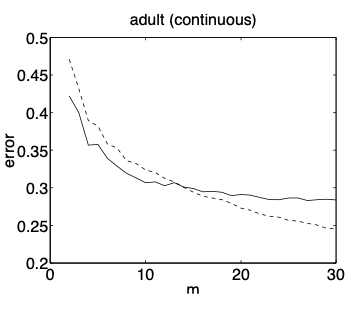
\includegraphics[scale=0.5]{figures/gen-disc}};
    		\node[fill=white,inner sep=1pt] (t1) at (2.5,3) {faster convergence};
         \draw[ultra thick,red,->] (t1) -- (7,2.5);
         \node[fill=white,inner sep=1pt] (t2) at (13,4.5) {higher asymptotic error};
         \draw[ultra thick,red,->] (t2) -- (10.5,2);
\end{tikzpicture}

Solid line: naive Bayes; dashed line: logistic regression.

\end{frame}

\end{document}
